\section{Conditional Deep Neural Networks}
\label{sec:conditional}
%Explain the conditional, pointing to the existing work. https://arxiv.org/pdf/1509.08971.pdf

%Identify any issues/drawbacks with this approach. How much information/confidence can be derived?
%Will interpretability be an issue and how much extra information be gathered from the task being partially completed?

Conventional deep neural networks (DNNs) have scaled greatly in depth, from 8 layers in AlexNet \cite{krizhevsky2012imagenet} to 1000 layers in ResNet-1001 \cite{he2016identity}. With the increase in size, the cost of implementing these very deep networks have increased as well. In order to determine the classification result, the input is processed through all the layers of the DNN, thereby consuming a lot of time and effort. However, in real world, not all inputs are made equal, and one can ideally design algorithms whose complexity is proportional to the difficulty of the input \cite{venkataramani2015scalable}. Such a design can provide both energy efficiency and speed up. Conditional Deep Learning \cite{panda2017energy, panda2016conditional} is a technique of augmenting deep neural networks with linear classifiers at the output of intermediate layers, that gives the user the control to conditionally activate the deeper layers of the network. 

In a Conditional Deep Learning network (CDLN), there are conditional exits added to the network after every few layers. As shown in Fig. \ref{fig:CDL-1}, when an input is presented to the network, the first linear classifier outputs the classification probability of the image. If the classifier has a strong confidence, that is the maximum output is beyond a threshold, then the network assigns the corresponding label to the input. If the confidence value is lower than threshold, then the next layers are activated and we move to the next classifier. These linear classifiers can be trained in tandem while training the whole network, or can be trained separately after the network is fully trained. 

\begin{figure}[h]
\centering
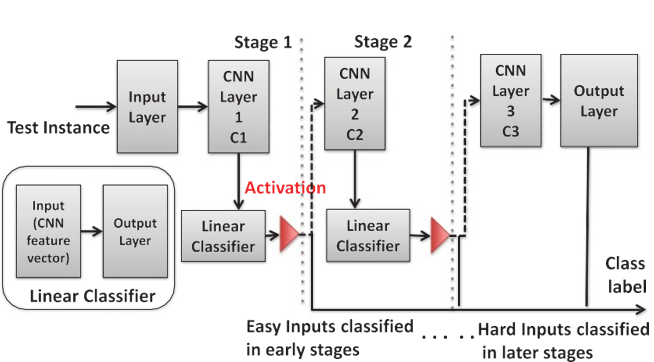
\includegraphics[width=0.45\textwidth]{CDL_1.png}
\caption{Conditional Deep Learning Network (CDLN) with linear classifiers added at the convolutional layers whose output is monitored to decide if classification can be terminated at current stage or not.} \label{fig:CDL-1}
\end{figure}

CDLN \cite{panda2017energy} offers $1.84\times$ improvement in energy in comparison to traditional implementation for MNIST on LeNet-5 \cite{lecun1998gradient}, which increases to $4.96\times$ for TinyImagenet implemented on ResNet-50 \cite{he2016deep}. Along with energy improvements, CDLN also offers significant improvement in inference time. As the whole network doesn't need to be activated for all the examples, average inference time per example reduces. It is reported in \cite{panda2017energy}, that CDLN implementation speed up the inference by $4.24\times$ for MNIST and $1.71\times$ for TinyImagenet. 

For a resource-constrained environment, CDLN offers an unique solution, that has both energy and timing improvements. In \cite{parsa2017staged}, conditional deep learning is used to implement staged inference for fast real time applications. For applications involving distributed intelligence, CDLN offers a framework that can be split up and deployed across edge and cloud. A low power system with low compute capabilities can be used to execute the the initial layers of the network. The linear classifier at the end of the first stage can provide us with some information regarding the input with a certain degree of confidence. In situations where the confidence of the edge is low, the data can be transmitted to the cloud to be processed by the remaining layers of the network. 












